\subsection{Database Design}

This section presents the database design of aBridgeAI through three views: the Entity-Relationship Diagram, the logical design, and the physical design. Together, these views describe how system data is structured, related, and implemented.
\subsubsection{Entity-Relationship Diagram}

The ERD provides a high-level view of the main entities in the system and the relationships between them.

\begin{figure}[H]
    \centering
    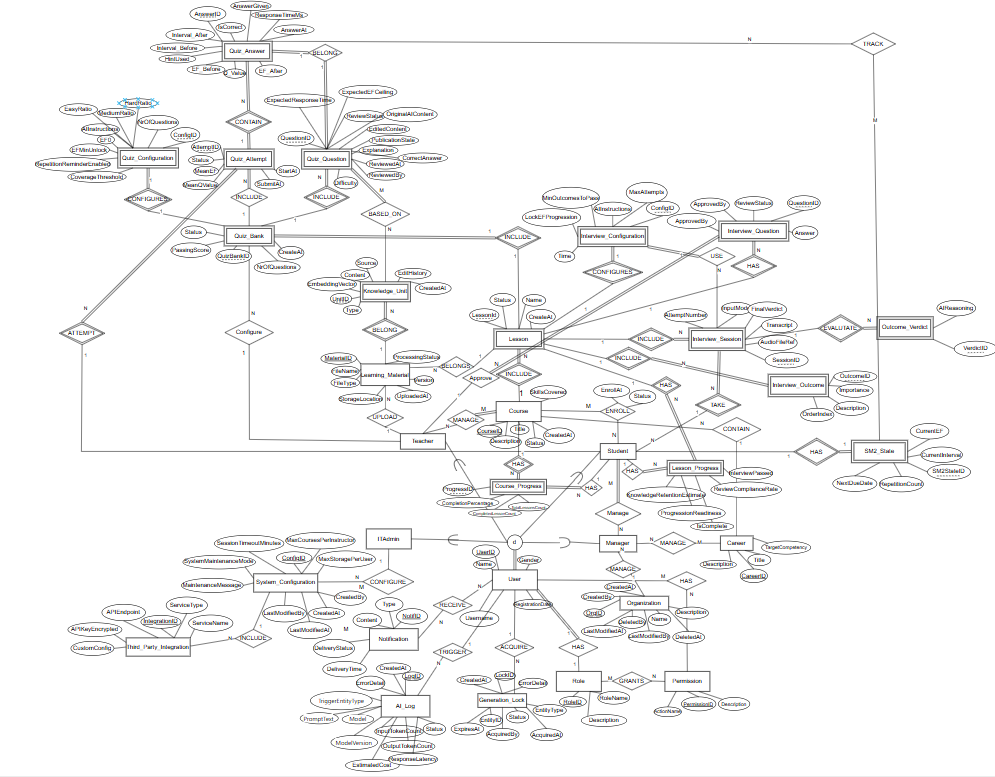
\includegraphics[width=\textwidth]{graphics/db-diagrams/ERD.png}
    \caption{Entity-Relationship Diagram}
    \label{fig:erd}
\end{figure}

\subsubsection{Logical Database Design}


\begin{figure}[H]
    \centering
    % Replace with logical database design image
    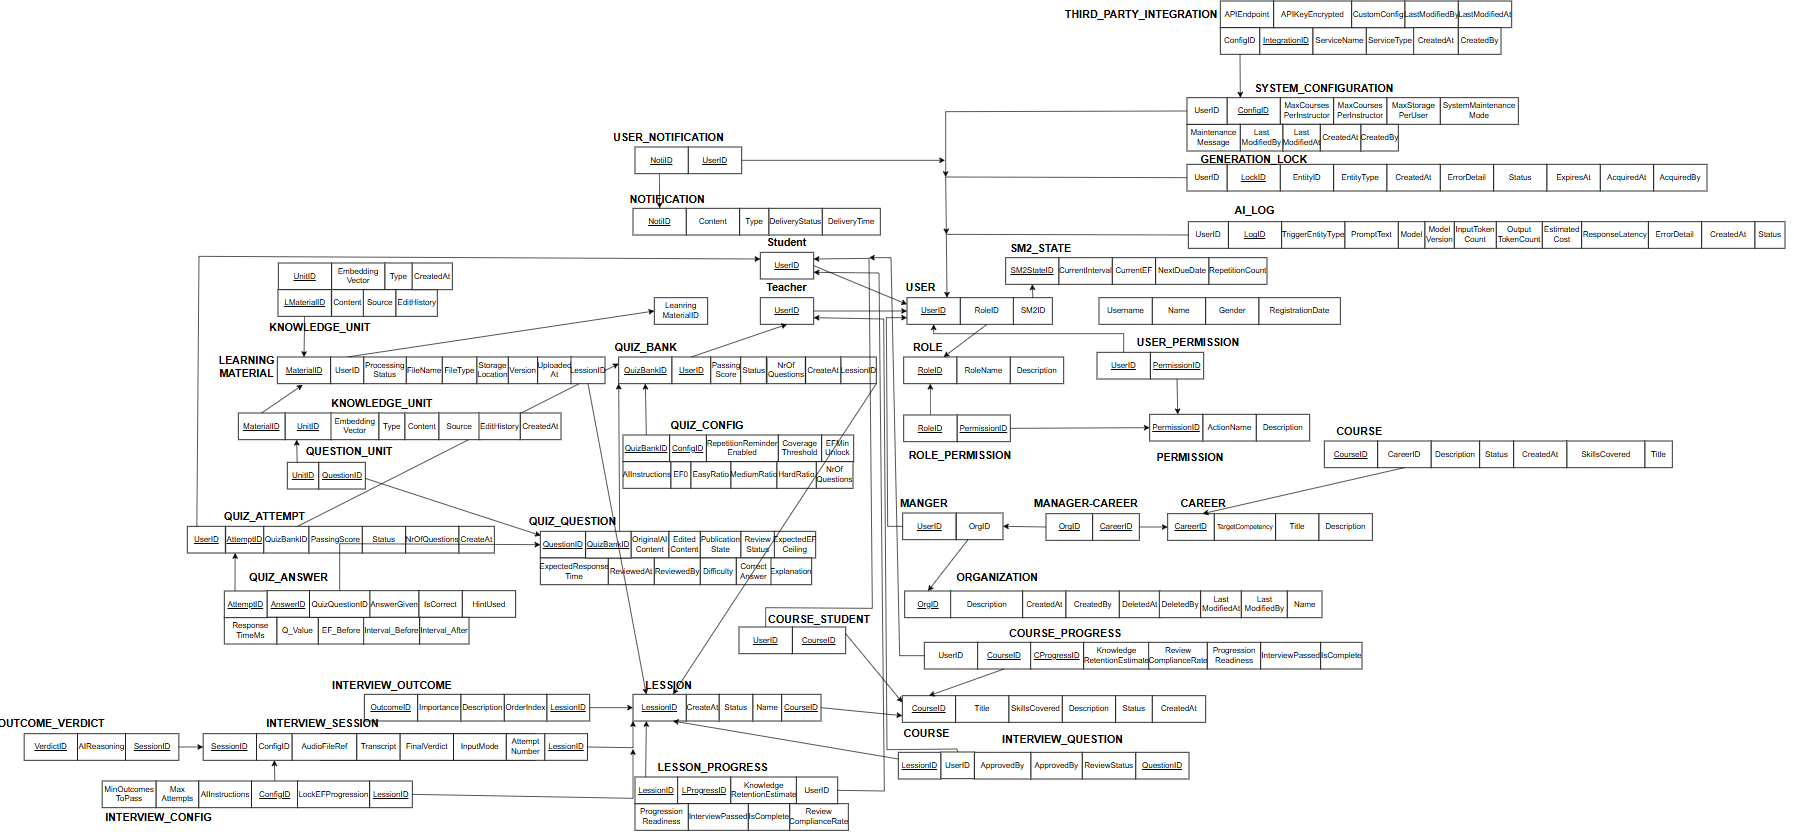
\includegraphics[width=\textwidth]{graphics/db-diagrams/LOGICAL_DESIGN.png}
    \caption{Logical Database Design}
    \label{fig:logical-db-design}
\end{figure}

\subsubsection{Physical Database Design}

\begin{figure}[H]
    \centering
    % Replace with physical database design image
    \includegraphics[width=\textwidth]{graphics/db-diagrams/PHYSICAL_DESIGN.pdf}
    \caption{Physical Database Design}
    \label{fig:physical-db-design}
\end{figure}